%!TeX program = lualatex
\documentclass[titlepage]{article}
\usepackage{../Head}
\usepackage[T1]{fontenc}
\usepackage{mathptmx}
\usepackage{bigints}
\graphicspath{.}
\begin{document}
\fancyhf{}
\fancyhead[RO,R]{Advanced Calculus 420}
\fancyhead[LO,L]{Dakota Wicker}
\fancyhead[CO,C]{Homework XI}
\cfoot{\thepage}

\begin{problem}{1}
Show that
$$ \vec{I}(t) = \vec{X} - s\vec{T}$$
\end{problem}
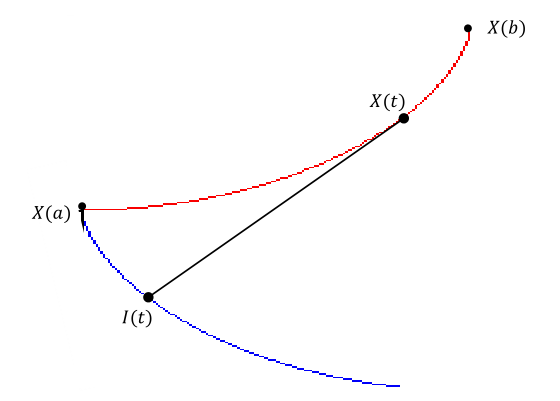
\includegraphics[scale=.5]{curves.png}
\begin{solution}
It is important to see in the diagram that the line created between ${X}(t)$ and ${I}(t)$ is the same length as the arc length between ${X}(a)$ and ${X}(t)$ which is equal to $s(t)$. Notice that the line is also in the opposite direction of the tangent vector at ${X}(t)$ since the function is increasing from $a\leq t\leq b$. This line can be written as $-s\vec{T}(t)$ because $\vec{T}(t)$ is the tangent unit vector and we multiply by $-1$ because the line is in the opposite direction. Then we multiply by $s(t)$ because that is its magnitude or length. Now, since $\vec{X}(t)$ has its tail where $-s\vec{T}(t)$ has its head the sum is a vector from $\vec{X}(a)$ to $\vec{I}(t)$ which draws the blue path. In other words, this shows that $\vec{I}(t) = \vec{X}(t)+ (-s\vec{T}(t)) = \vec{X}(t) -s\vec{T}(t)$.
\end{solution}

\begin{problem}{2}
Show that the involute of the section of cycloid given by
$$x = a(\theta - \sin(\theta))$$
$$y = a(1 - \cos(\theta))$$
from the point $X(0) = (0,0)$ is given by
$$ I(t) = \begin{bmatrix}a(\theta + \sin(\theta)) \\ a(3 + \cos(\theta)) \end{bmatrix}, -\pi \leq \theta \leq 0$$
\end{problem}

\begin{solution}
Since I have shown that $\vec{I}(t) = \vec{X}(t) -s(t)\vec{T}(t)$, I will use this fact. I am given that 
$$x = a(\theta - \sin(\theta))$$
$$y = a(1 - \cos(\theta))$$
$$ -\pi \leq \theta \leq 0$$
Using substitution I get
$$\vec{I}(\theta) = \vec{X}(\theta) - s(\theta)\vec{T}(\theta) = \begin{bmatrix} a(\theta - \sin(\theta)) \\ a(1 - \cos(\theta)) \end{bmatrix} - s(\theta)\vec{T}(\theta)$$
Then, the arclength is defined as $$s(\theta) = \bigintss_{\theta = -\pi}^{\theta}\sqrt{\left(\frac{dx}{d\theta}^2\right) + \left(\frac{dy}{d\theta}^2\right)} \ d\theta$$
$$=  \bigintss_{\theta=-\pi}^{\theta}\sqrt{(a- a \cos(\theta))^2 + (a\sin(\theta))^2}$$
$$=  \bigintss_{\theta=-\pi}^{\theta}\sqrt{a^2 - 2a^2\cos(\theta) + (a\cos(\theta))^2 + (a\sin(\theta))^2}\ d\theta$$ 
$$=\bigintss_{\theta=-\pi}^{\theta}\sqrt{2a^2 - 2a^2\cos(\theta)} \ d\theta $$
$$= \bigintss_{\theta=-\pi}^{\theta}\sqrt{2a^2(1-\cos(\theta))}\ d\theta $$
$$= \sqrt{2a}\bigintss_{\theta=-\pi}^{\theta}\sqrt{1-\cos(\theta)} \ d\theta$$
$$= 2a\bigintss_{\theta=-\pi}^{\theta}\sqrt{2\sin^2(\frac{\theta}{2})} \ d\theta$$
$$= 2a \bigintss_{\theta=-\pi}^{\theta}\left|\sin(\frac{\theta}{2})\right| \ d\theta = 2a\bigintss_{\theta=-\pi}^{\theta}\sin(\frac{\theta}{2}) \ d\theta = 4a\cos(\frac{\theta}{2})$$
Plugging this function into the equation I get
$$\vec{I}(t) = \begin{bmatrix} a(\theta - \sin(\theta)) \\ a(1 - \cos(\theta)) \end{bmatrix} - 4a\cos(\frac{\theta}{2})\vec{T}(t)$$
By defintion, $\vec{T}(t) = \frac{\frac{d\vec{X}}{d\theta}}{\left|\frac{d\vec{X}}{d\theta}\right|}$. So, differentiating and plugging in values I get 
$$\vec{T}(t) = \begin{bmatrix} \frac{a(1-\cos(\theta))}{-2a\sin(\frac{\theta}{2})} \\ \frac{a\sin(\theta)}{-2a\sin(\frac{\theta}{2})}\end{bmatrix}$$
Finally, substituting all values I get
$$\vec{I}(t) = \begin{bmatrix} a(\theta - \sin(\theta)) \\ a(1 - \cos(\theta)) \end{bmatrix} - 4a\cos(\frac{\theta}{2})  \begin{bmatrix} \frac{a(1-\cos(\theta))}{-2a\sin(\frac{\theta}{2})} \\ \frac{a\sin(\theta)}{-2a\sin(\frac{\theta}{2})}\end{bmatrix} =\begin{bmatrix}a(\theta + \sin(\theta)) \\ a(3 + \cos(\theta)) \end{bmatrix}.$$
\end{solution}

\begin{problem}{3}
Use substitution $\alpha = \theta + \pi$ to show that this involute is a section of cycloid shifted by the vector $$\begin{bmatrix}-\pi a \\ 2a\end{bmatrix}$$
\end{problem}
\clearpage
\begin{solution}
\begin{align*}
\vec{I}(t) &= \begin{bmatrix} a(\alpha-\pi) + \sin(\alpha - \pi) \\ a(3+\cos(\alpha-\pi))\end{bmatrix}\\
 &= \begin{bmatrix} a(\alpha - \pi) + \sin(\alpha)\cos(\pi) - \cos(\alpha)\sin(\pi) \\ a(3+(\cos(\alpha)\cos(\pi) + \sin(\alpha)\sin(\pi)))\end{bmatrix}\\
 &= \begin{bmatrix}a(\alpha - \pi) - \sin(\alpha) \\ a(3-\cos(\alpha)) \end{bmatrix}\\
 &= \begin{bmatrix} \alpha^2-\alpha\pi-a\sin(\alpha) \\ 3a-a\cos(\alpha)\end{bmatrix} \\
 &= \begin{bmatrix}a(\alpha - \sin(\alpha)) \\ a(1-\cos(\alpha))\end{bmatrix} + \begin{bmatrix}-\pi a \\ 2a \end{bmatrix}, 0 \leq \alpha \leq \pi
\end{align*}
\end{solution}

\end{document}